\section{Works Done}
\label{sec:worksDone}
\subsubsection{Mechanic Part}
This week the door is tested by using cutting cardboard. As mentioned in the previous reports, we have make a door using the idea of salts. This can be seen on Fig 1.

\begin{figure}[h]
    \centering
    \begin{subfigure}[b]{0.49\linewidth}
        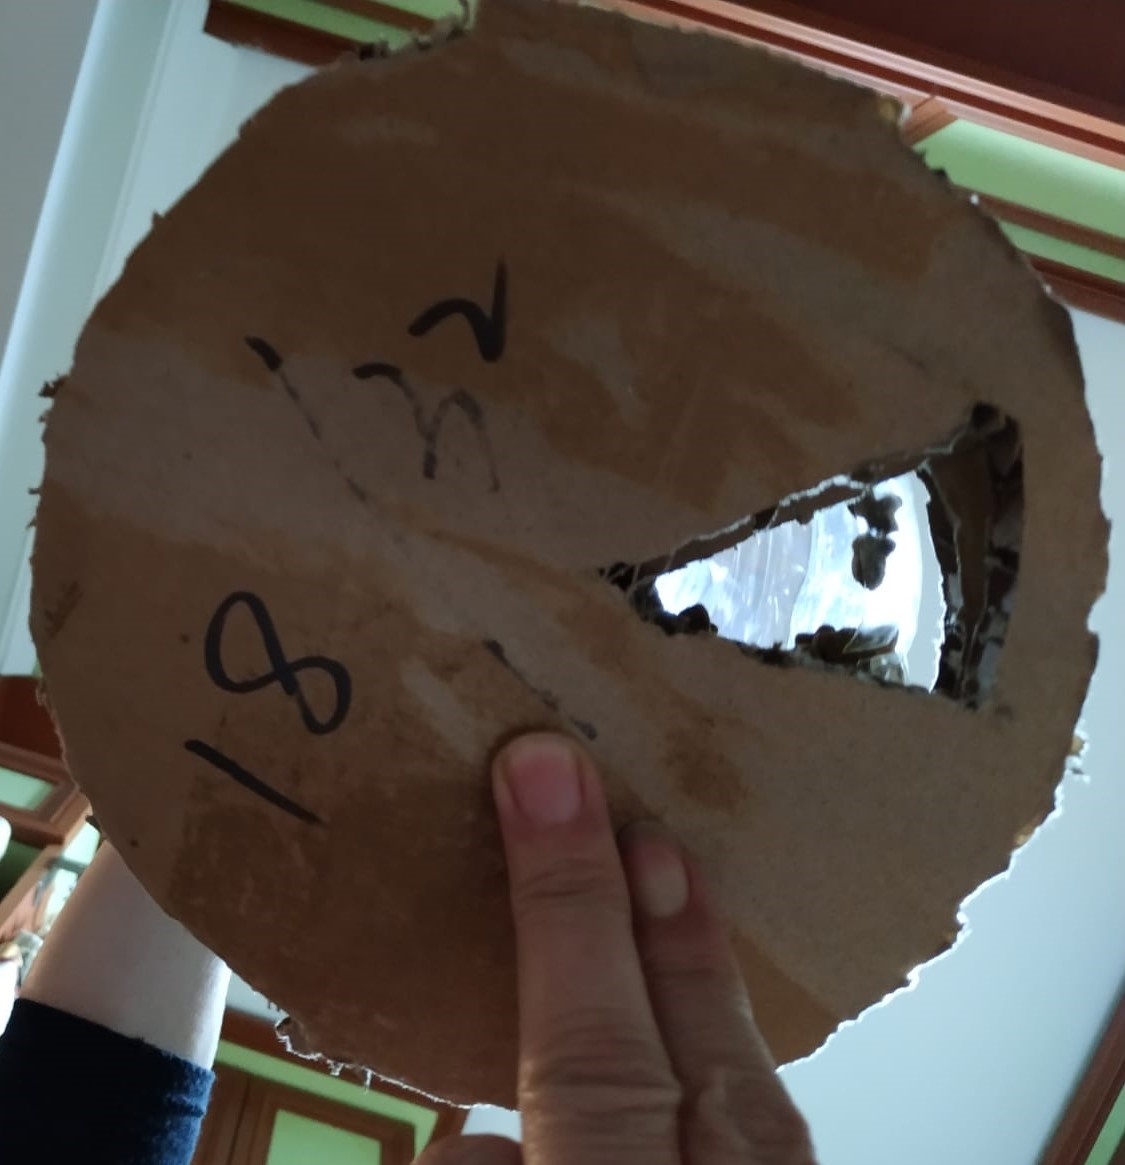
\includegraphics[width=\linewidth]{Mech2.jpeg}
        \caption{Bottom View}
        \label{fig:doga1}
    \end{subfigure}
    \begin{subfigure}[b]{0.49\linewidth}
        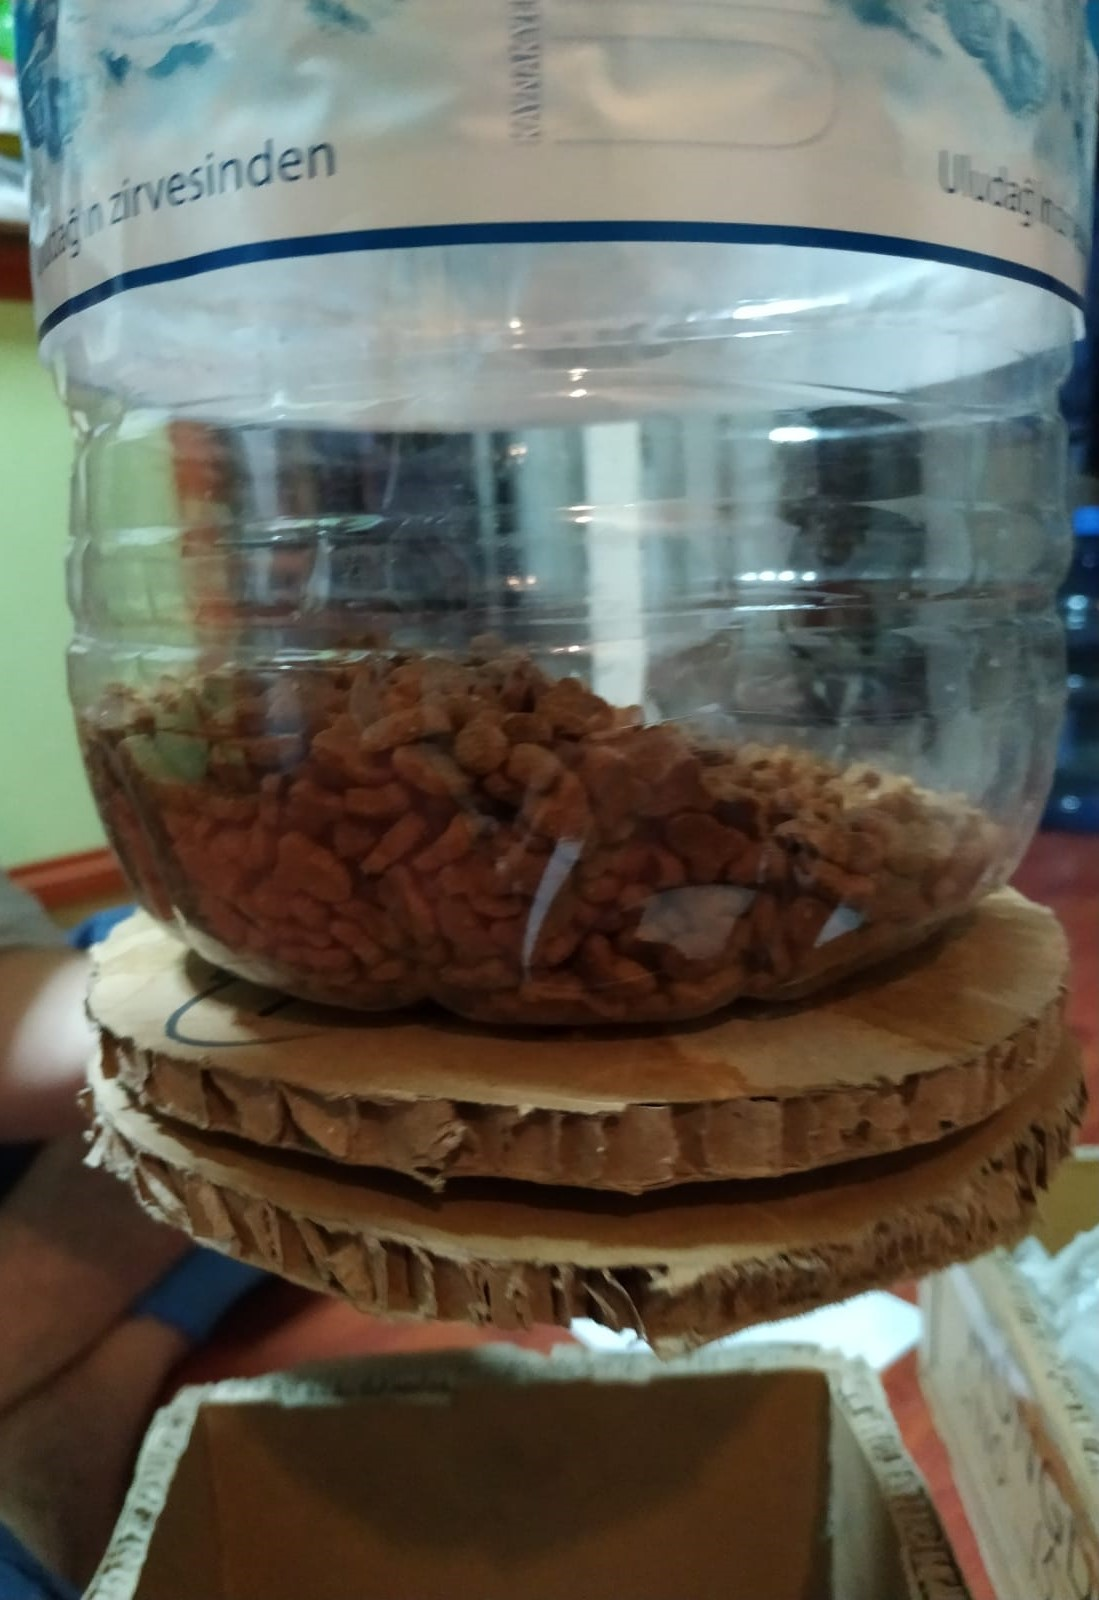
\includegraphics[width=\linewidth]{Mech3.jpeg}
        \caption{Top View}
        \label{fig:doga2}
    \end{subfigure}
  
\end{figure}

In order to rotate the lower cardboard one has to use a strong servo motor. Therefore some of the servo motors are examined like:
\begin{itemize}
    \item TowerPro MG995R
    
    Torque: 9.4kg-cm
    
    Speed: 0.20sec/60degree
    
    Size: 40.7×19.7×42.9mm
    
    Cost: 35TL
    
    \item TowerPro Mg996R
    
    Torque: 9.4kg-cm(4.8v)-11kg-cm(6.0v)
    
    Speed: 0.19sec/60 degree(4.8v)-0.15sec/60 degree(6.0v)
    
    Size: 40.9×20×42.7mm
    
    Cost: 36TL
    
    \item Futaba S3003
    
    Torque : 4.1kg.cm
    
    Speed : 0.23sec/60 degrees
    
    Size : 41 x 20 x 36mm
    
    Cost : 42 TL
\end{itemize}

These are called as high torque servos. First two servos look like as if they can rotate our cardboard. It looks like the lower cardboard will carry at most 600gr, while it's radius is 8cm. 
 9.4/16 = 0.58kg which is close to 600gr. 
 In addition to that one can also use gearbox to improve the torque but it is not desirable since it can create speed and design problems. 
 
 A meeting is conducted with the furnishes for the outer design and as soon as inner design is finished the exterior design will be ordered. 
 
 
 
\subsection{Software Framework and Computer Vision}
Works done in detail are given in detail below as items. In a general view, a working system is constructed and tested. The first time hardware - software - computer vision parts are interated together and tested.

\begin{itemize}
    \item Server client communication software is finished and integrated with the computer vision part with currently available features.
    \item Test of the parts individually are done and some optimization - corrections are made
    \item Real time performance is tested, results is given in the \ref{subsec:realTime} section for both present the current work done and create a reference
    \item Data-sets created from real time camera images and video capture
    \item YOLO integrated to the OpenCV is used
    \item Documentation is prepared for these parts for other uses
\end{itemize}


\subsection{Real Time Results}
\label{subsec:realTime}
In this section different kinds of results are given. Accuracy, 
TODO - tesleri yazmadim ekleyelim ama - accuracy eklemeli
\subsubsection{Classification Results}
Classification results are given in figure \ref{fig:classificationResults}.

\begin{figure}[h]
    \centering
    \begin{subfigure}[t]{0.49\linewidth}
    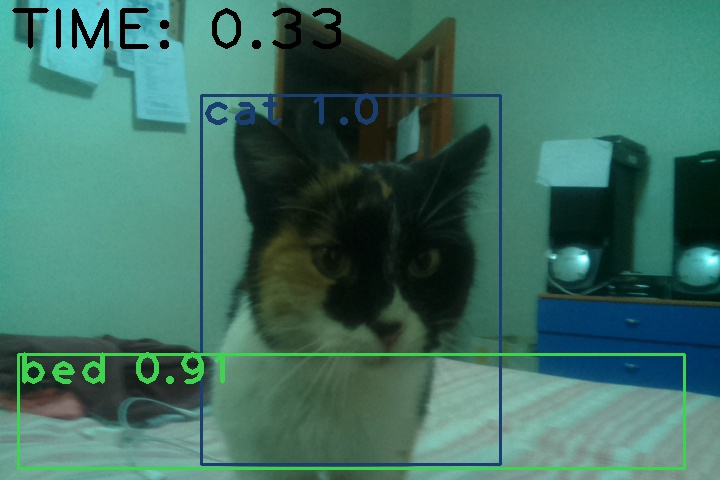
\includegraphics[width=\linewidth]{eserImg/sampleClassification1.jpg}
    \caption{Sample Classification 1}
    \label{fig:classificationSample1}
    \end{subfigure}
    \begin{subfigure}[t]{0.49\linewidth}
    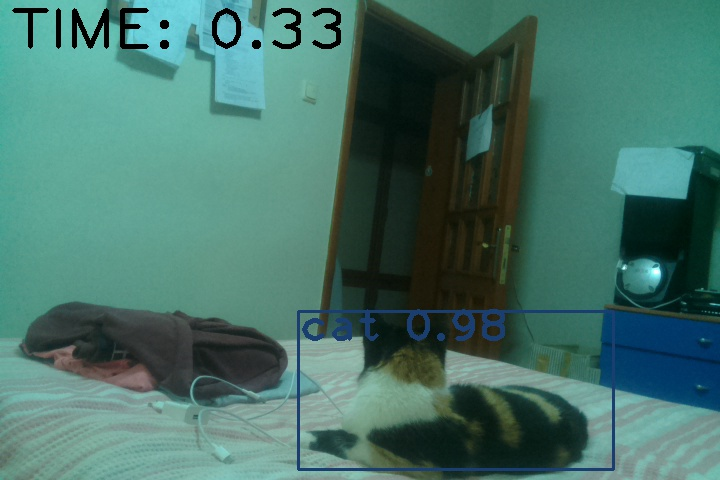
\includegraphics[width=\linewidth]{eserImg/sampleClassification2.jpg}
    \caption{Sample Classification 2}
    \label{fig:classificationSample1}
    \end{subfigure}
    \begin{subfigure}[t]{0.49\linewidth}
    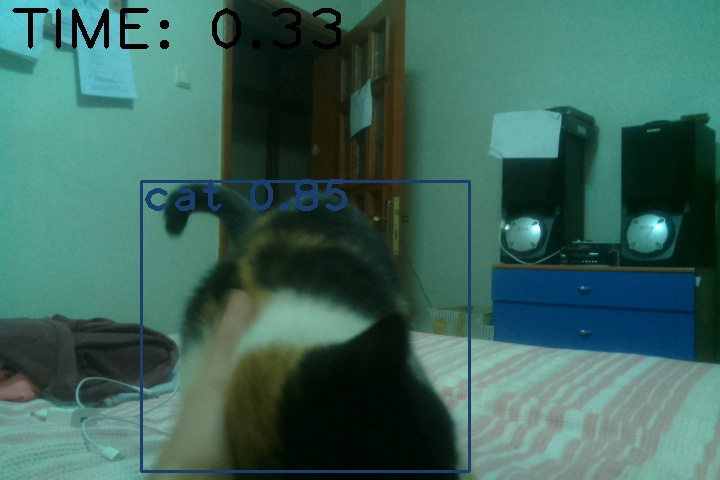
\includegraphics[width=\linewidth]{eserImg/sampleClassification3.jpg}
    \caption{Sample Classification 3}
    \label{fig:classificationSample1}
    \end{subfigure}
    \begin{subfigure}[t]{0.49\linewidth}
    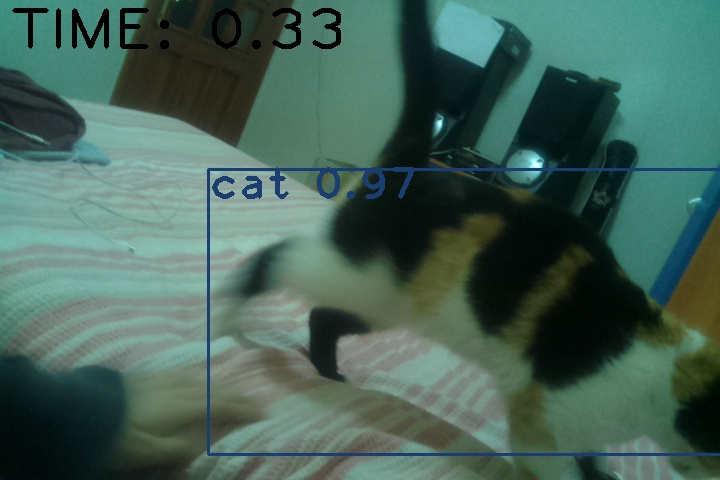
\includegraphics[width=\linewidth]{eserImg/sampleClassification4.jpg}
    \caption{Sample Classification 4}
    \label{fig:classificationSample1}
    
    \end{subfigure}
    
    \caption{Some Classification Results}
    \label{fig:classificationResults}
\end{figure}

\subsubsection{Response Time Results}

\subsubsection{CPU - Memory Usage}
\paragraph{Client Hardware Statistics}

\paragraph{Server Hardware Statistics}


\subsection{Discussion}
It is clear the system should be improved further by adding other parameters and techniques to eliminate wrong results, especially false positives!. Some of the methods we propose are given as follows:
\begin{itemize}
    \item Taking the most repeated result for the last 5 time frames
    \item Averaging the accuracy values given by OpenCV
    \item Building confidence intervals
    \item Mixture - Building confidence intervals dynamically depending on the first two techniques
\end{itemize}